\subsection{Liquidity Simulation Environment\label{section:lse}}

As part of building Mosaic \cite{MosaicFinance} we wanted to understand the nature of liquidity and how its allocation and movement means for the design of the system.
%
To that end, Composable Labs \cite{IntroducingMedium} built a Liquidity Simulation Environment (LSE) \cite{IntroducingMediumb}.

This software tool can simulate allocations of assets to vaults and assets moving around in the network.
%
It is modular and you can produce data in any form you want.
%
Currently, the LSE supports data generated from a truncated Gaussian, Geometric Brownian Motion (GBM), and data sampled from our 2021 September-October PoC run \cite{TestingMedium}.

The strategy layer allows for any liquidity allocation and movement approach to be defined. For example "move liquidity from vault X to vault Y when conditions Z is true".
%
An objective - which can also be defined in the LSE - useful for searching for the best strategy could be to optimize the liquidity distribution among the vaults so that any transfer can be supported.

Fee models, how much and simply how, to charge moving assets can be defined as well. In fact, we used the PoC in conjuncion with the LSE to decide the best fee model to use in the context of available data up to that point.

The LSE is built as a state-machine iterating through the simulated transfers changing the states of the vaults. Replenishment events can be triggered - for example: the Arbitrum vault needs liquidity from the Mainnet vault.

The LSE is also continuously improving. As more transfer data is received this gives us a unique insight into how Mosaic is used and the LSE can help fine-tune our network to achieve an optimal user experience by having maximum availability.

\subsubsection{Simulating Data}

The LSE supports generating simulated transfer/usage data. We use this to model behavior of network usage and based on that make decisions on how to distribute liquidity.

We support generating data from a truncated Gaussian distribution. We sample a timeline and on that a set of hypothetical cross-chain cross-layer moves from this distribution with given mean and standard deviation.
%
We also support generating data from a Geometric Brownian Motion.
%
The moves or transactions $N_t$ (amount of \$) from one vault to another, at time $t$, following a GBM model, are described by the following stochastic differential equation (SDE)
\begin{equation}
\frac{d N_t}{dt} = \mu N_t + \sigma N_t\frac{dW_t}{dt}, 
\end{equation}
with $\mu$ being a drift term, $\sigma$ the volatility, both assumed to be constants and $W_t$ is a Brownian motion stochastic process. The analytical solution of the above SDE at time t, given initial condition $N_0$, is known to be 
\begin{equation}
\label{eq:gbm_solution}
N_t = N_0 \exp\left[ \left(\mu - \frac{\sigma^2}{2}\right) t + \sigma W_t\right],
\end{equation}
which by definition is always strictly positive. A key property of the solution, important for our LSE use, is that the solution asymptotically goes to infinity when $\mu > \frac{1}{2}\sigma^2$, it goes to $0$ when $\mu < \frac{1}{2}$ and it fluctuates between zero and arbitrarily large values when $\mu = \frac{1}{2}\sigma^2$, therefore for most of our cases we will be using $\mu = \frac{1}{2}\sigma^2$. Fig. \ref{fig:gbm} shows two random simulation of eq. (\ref{eq:gbm_solution}) for the $N_0 = \$2000$, $\sigma=2$ and $N_0=\$1500$, $\sigma=1$ respectively. Note that the same initial and volatility values have also been used in our simulations below to simulate moves from Polygon to Arbitrum vaults and vice versa.
%
\begin{figure}[h]
    \centering
    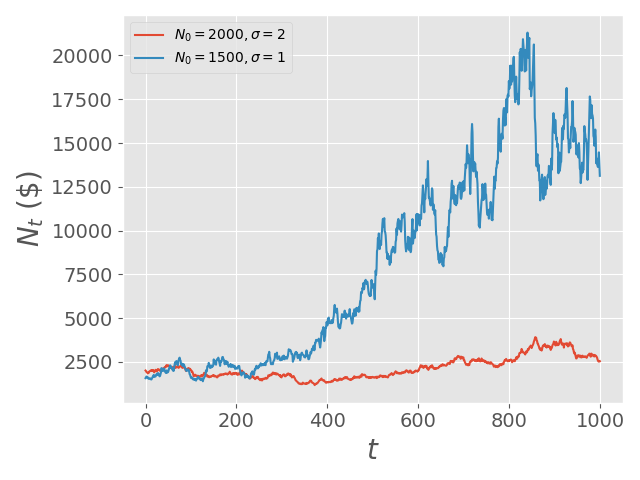
\includegraphics[width=0.5\textwidth]{images/gbms.png}
    \caption{Simulation of Geometric Brownian motion data in Composable's Liquidity Simulation Environment (LSE).}
    \label{fig:gbm}
\end{figure}
%

These results guided us to an answer on two key questions to kick off the Mosaic PoC: First, how much liquidity should be assigned in total and then how much should be assigned to each network? Second, which transfer fee model should we initially use?

These results guided us to decide on a good initial fee model to use for the Mosaic PoC. We then ran the PoC with that model, collected the data, and optimized the model to its final form. More on that in Sec.~(\ref{sec:feemodel}).

\subsubsection{Mosaic Fee Model\label{sec:feemodel}}

One of the first use-cases of the LSE was deciding which fee model to use for Mosaic.
%
Fees are charged when funds are moved between networks. The question of which fee model to go with is key to a successful deployment.

First, guided by Occam's razor \cite{WhatRazor} we picked a simple functional form and let the fee model follow a linear form capped by a maximum fee ensuring that nobody, no matter how much they move across Mosaic, is charged more than a certain percent.

For most transfers, and for practically all retail transfers, users move along the linear part close to the origin.
%
To ensure a safe network, we implemented a minimum fee as well distributing rewards to maintainers. Let $x$ denote the liquidity moved as percent of available liquidity in the origin vault. For example, if I move 10 ETH in a vault with 200 ETH $x=5$\%. Let $y$ be the fee charged in percent. The Mosaic fee model is then determined by the two points $(x,y)=(0,0.25)$ and $(x,y)=(30,5)$.

The Mosaic PoC was run with this model and based on the data the two points were optimized to balance use and network safety (indirectly via rewards collected from fees).

We have three free parameters in our fee model:
\begin{itemize}
    \item the liquidity-\% at which the maximum fee kicks in (also called $a$)
    \item the maximum fee \% to charge
    \item the minimum fee \% to charge
\end{itemize}

In the PoC these parameters were: 40\%, 4\%, and 0.25\%, respectively. For ease, we will denote this parameter set in the format (40, 4, 0.25).

The PoC transfer data is visualized in Fig.~(\ref{fig:pocdatavis}).
%
\begin{figure}
    \centering
    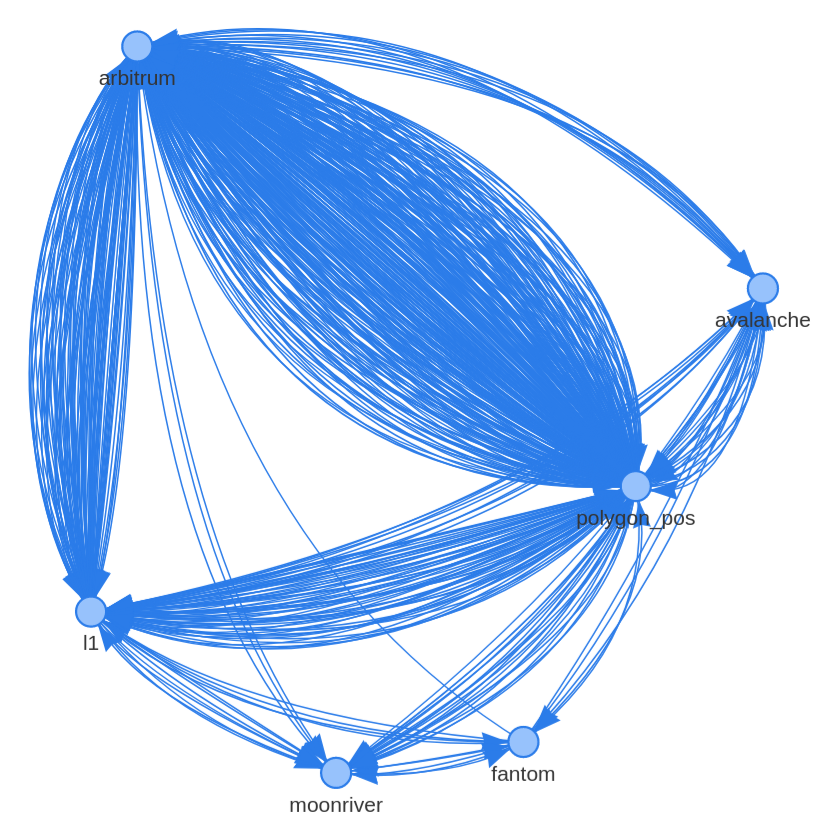
\includegraphics[width=0.6\textwidth]{images/mosaic/pocdata.png}
    \caption{Visualizing the Mosaic PoC bridge transfer data. Each network supported by Mosaic in the PoC is a node and edges represent transfers between the networks. Note that Arbitrum and Polygon were there from the beginning and other networks were added later. Thus, edges are not normalized by time and surely does not imply "popularity" of a network.}
    \label{fig:pocdatavis}
\end{figure}
%
We next visualize the fees charged for the PoC data in Fig.~(\ref{fig:pocdatafees}).
%
\begin{figure}
    \centering
    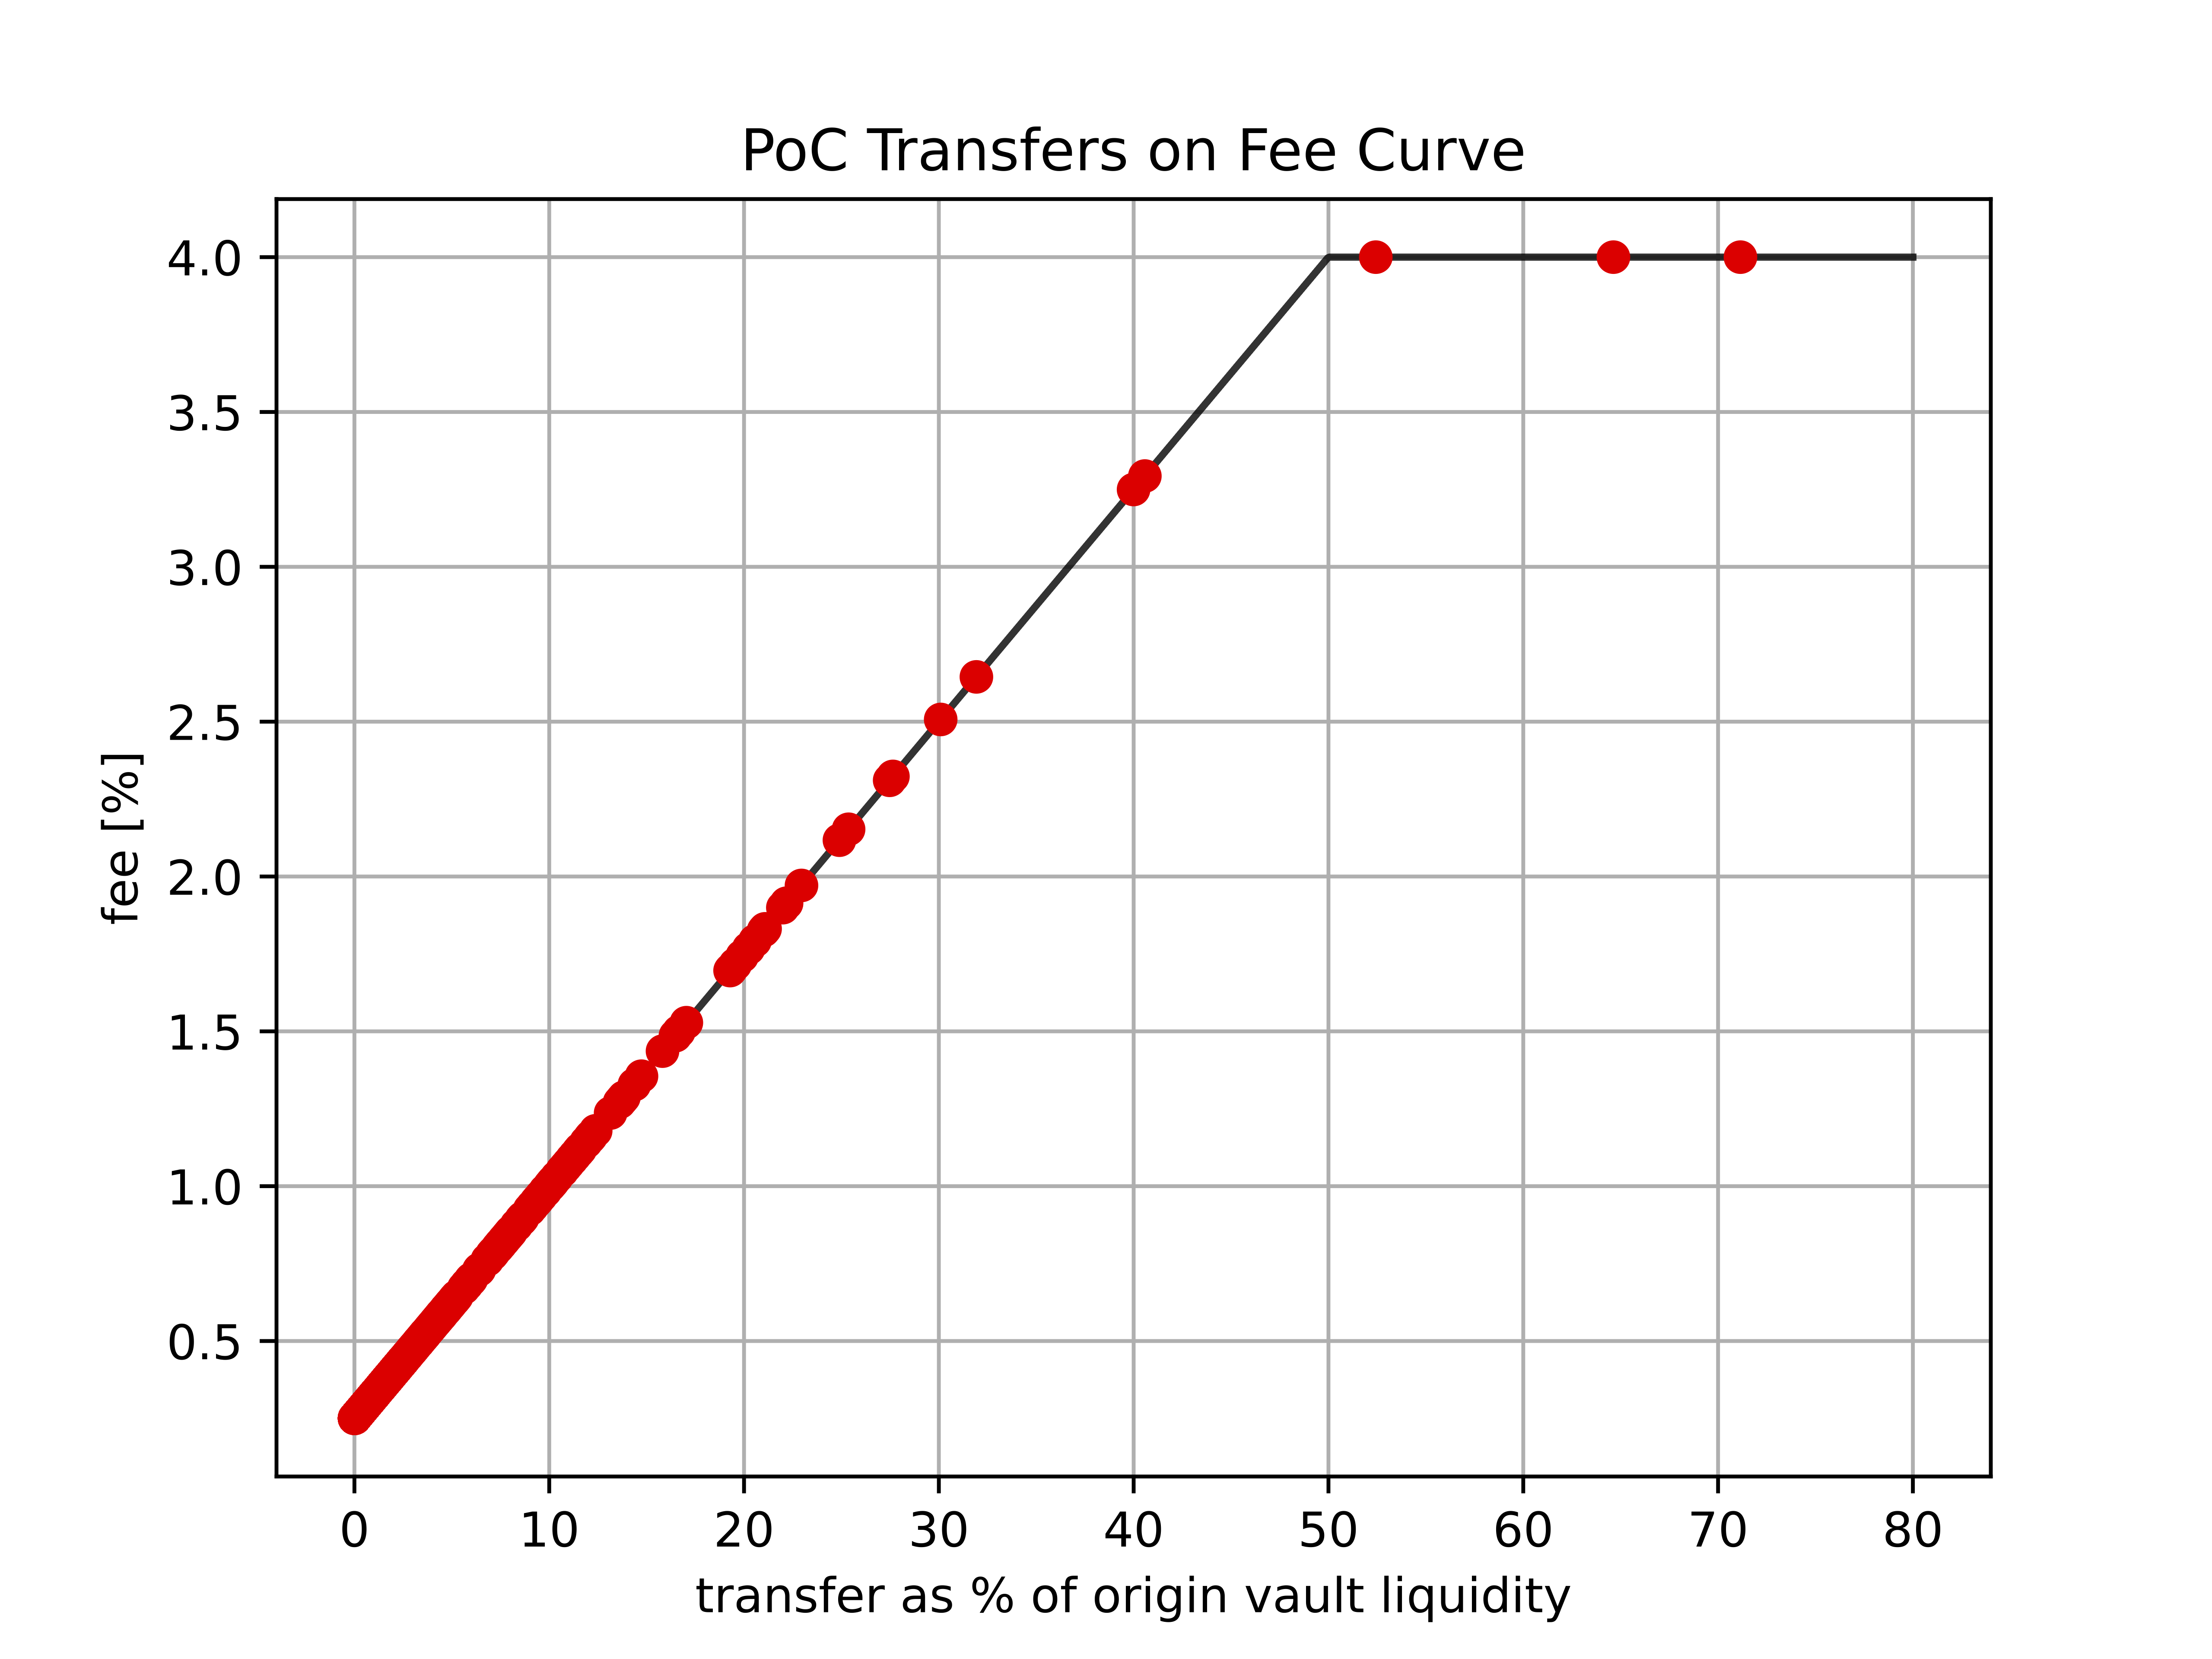
\includegraphics[width=0.8\textwidth]{images/mosaic/poc_transfer_on_fee_curve.png}
    \caption{Fee charged vs transfer amounts as percent of available liquidity in the origin vault. For example, if 10 wETH is transferred from a vault on Arbitrum with 1000 wETH it would show up at $x=10$\%. The y-axis shows the fee charged for the transfer. For the PoC vaults were on the order of \$100-200k at the beginning of the PoC. The exact numbers for each token (which in turn was distributed across multiple networks like Arbitrum and Polygon) are available here: \href{https://mosaic.composable.finance/earn}{TVLs for Mosaic} (accessed November 12, 2021).}
    \label{fig:pocdatafees}
\end{figure}
%
To decide on a good set of parameters, we next compare this to bridges seen in the general cross-ledger community.

We find that some operators charge a fixed 0.5\% for all transfers, higher than the average Mosaic PoC case.

Other operators charge different fees depending on whether you are leaving Ethereum or arriving from another chain. Some charge a fixed dollar amount and others a percentage with minimum and maximum dollar amounts.

Some operators do not charge a fee but instead charge a ``hidden fee" by quoting a given ``transfer rate". They also create bi-directional fees (mainnet to polygon is different than polygon to mainnet).
%
Other operators charge a fee that is a multiple of the destination network fee.

And so on.

Given this landscape of fees the following parameters were chosen: (30, 4, 0.25) (liquidity-\% at which max fee kicks in, maximum fee \% to charge, minimum fee \% to charge, respectively).
%
This optimized fee curve is shown in Fig.~(\ref{fig:pocdatafeesopt}).
%
\begin{figure}
    \centering
    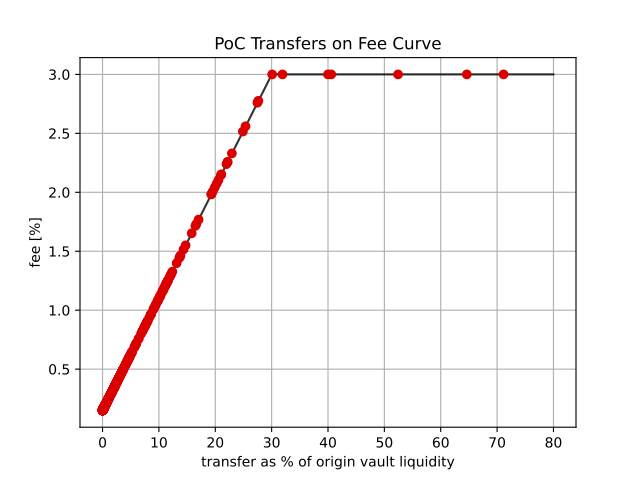
\includegraphics[width=0.8\textwidth]{images/mosaic/poc_optimized.png}
    \caption{The PoC data transformed to the optimized fee curve with parameters (30, 4, 0.25).}
    \label{fig:pocdatafeesopt}
\end{figure}
%

\subsubsection{Continuous Improvement}

With the LSE we can continuously collect data from the operation of Mosaic and periodically revisit the fee model parameter settings.
%
This introduces us, as shown, to a purely data driven approach to determine this. We would use Graph QL \cite{GraphQLAPI} to collect data from the Mosaic network, compute the fees/revenues collected and ensure that we stay within a certain band of expected and allowable values. We make this check once a week.
%
If we stray away from expected values, we modify the parameters if necessary based on a data review.
